% LaTeX-Folienvorlage erstellt von Mathias Magdowski (mathias.magdowski@ovgu.de)
% veröffentlicht unter Creative-Commons-Lizenz mit Namensnennung und Weitergabe unter gleichen Bedingungen 4.0 International (CC BY-SA 4.0, https://creativecommons.org/licenses/by-sa/4.0/deed.de)
% basierend auf der PowerPoint-Vorlage von http://bit.ly/ppt-digiPH (Stand: Anfang April 2018)

% Beamer-Klasse
\documentclass{beamer}

% Pakete laden
% Paket für Deutsche Sprache (Übersetzungen von Chapter zu Kapitel, 
% richtige Umlaute, richtige % Silbentrennung)
% siehe auch http://de.wikipedia.org/wiki/Babel-System
\usepackage[ngerman]{babel}

% Eingabecodierung, deutsche Umlaute oder die akzentuierten Zeichen sind verfügbar 
% und können direkt eingegeben werden
% siehe auch http://de.wikipedia.org/wiki/UTF8
\usepackage[utf8]{inputenc}

% Ausgabeschriftart von LaTeX festlegen
% siehe auch http://de.wikibooks.org/wiki/LaTeX-Schnellkurs:_Erste_Schritte
\usepackage[T1]{fontenc}

% Standardpfad für Grafiken
\graphicspath{{logos/}{bilder/}{fotos/}}

% Paket zum Erstellen von Plots mit TikZ
\usepackage{pgfplots}
% immer die neueste Version benutzen
\pgfplotsset{compat=newest}
% Verbindung von Linien durch eine schräge Kante
\pgfplotsset{every axis/.append style={line join=bevel}}
% Formatvorlage für Präsentationen
\mode<beamer>{
	\pgfplotsset{
		beamer/.style={
			width=0.8\textwidth,
			height=0.45\textwidth,
			legend style={font=\scriptsize},
			tick label style={font=\footnotesize},
			label style={font=\small},
			max space between ticks=28,
		}
	}
}
\mode<handout>{
	\pgfplotsset{
		beamer/.style={
			width=0.8\textwidth,
			height=0.45\textwidth,
			legend style={font=\scriptsize},
			tick label style={font=\footnotesize},
			label style={font=\small},
			max space between ticks=25,
		}
	}
}
\mode<article>{
	\pgfplotsset{
		beamer/.style={
			width=0.8\textwidth,
			height=0.45\textwidth,
			max space between ticks=35,
		}
	}
}
% neue Größenvorlage für zwei Plots nebeneinander anlegen
\pgfplotsset{
	scriptsize/.style={
		width=0.34\textwidth,
		height=0.1768\textwidth,
		legend style={font=\scriptsize},
		tick label style={font=\scriptsize},
		label style={font=\footnotesize},
		title style={font=\footnotesize},
		every axis title shift=0pt,
		max space between ticks=25,
		every mark/.append style={mark size=7},
		major tick length=0.1cm,
		minor tick length=0.066cm,
	}
}
\pgfplotsset{
	small/.style={
		width=6.5cm,
		height=,
		tick label style={font=\footnotesize},
		label style={font=\small},
		legend style={font=\footnotesize},
		max space between ticks=30,
	}
}
% Legendeneintrage standardmäßig links ausrichten
\pgfplotsset{legend cell align=left}
% Hauptgitternetz zeichnen
\pgfplotsset{xmajorgrids}
\pgfplotsset{ymajorgrids}
% Anzahl der kleinen Teilstriche zwischen zwei großen Teilstrichen
%\pgfplotsset{minor x tick num={3}}
%\pgfplotsset{minor y tick num={3}}
% feines Gitternetz zeichnen
%\pgfplotsset{xminorgrids}
%\pgfplotsset{yminorgrids}
% nur nach den Achsen skalieren
\pgfplotsset{scale only axis}
% Farben wie in MATLAB definieren
\definecolor{matlab1}{rgb}{0,0,1}
\definecolor{matlab2}{rgb}{0,0.5,0}
\definecolor{matlab3}{rgb}{1,0,0}
\definecolor{matlab4}{rgb}{0,0.75,0.75}
\definecolor{matlab5}{rgb}{0.75,0,0.75}
\definecolor{matlab6}{rgb}{0.75,0.75,0}
\definecolor{matlab7}{rgb}{0.25,0.25,0.25}
% Farbreihenfolge wie in MATLAB definieren
\pgfplotscreateplotcyclelist{matlab}{
	{matlab1,solid},
	{matlab2,dashed},
	{matlab3,dashdotted},
	{matlab4,dotted},
	{matlab5,densely dashed},
	{matlab6,densely dashdotted},
	{matlab7,densely dotted}% dies unterdrückt einen Fehler
}
% Farbreihenfolge wie in MATLAB benutzen
\pgfplotsset{cycle list name=matlab}
% Farbreihenfolge von pgfplots benutzen
%\pgfplotsset{cycle list name=color list}
% nur Graustufen benutzen
%\pgfplotsset{cycle list name=linestyles}
% Strichstärke auf 1pt festlegen
\pgfplotsset{every axis plot/.append style={line width=1pt}}
% für deutsche Dokumente ein Komma benutzen
\addto\extrasngerman{\pgfplotsset{/pgf/number format/.cd,set decimal separator={{{,}}}}}
% ein halbes Leerzeichen als Tausendertrennzeichen benutzen
%\pgfplotsset{/pgf/number format/.cd,1000 sep={\,}}
% kein Tausendertrennzeichen verwenden
\pgfplotsset{/pgf/number format/.cd,1000 sep={}}
% Zahlen kleiner als 0.1 auch im fixed-Format ausgeben
\pgfplotsset{/pgf/number format/.cd,std=-2}
% neue Positionen für Legenden anlegen
\pgfplotsset{/pgfplots/legend pos/north/.style={/pgfplots/legend style={at={(0.50,0.97)},anchor=north}}}
\pgfplotsset{/pgfplots/legend pos/south/.style={/pgfplots/legend style={at={(0.50,0.03)},anchor=south}}}
\pgfplotsset{/pgfplots/legend pos/east/.style={/pgfplots/legend style={at={(0.97,0.50)},anchor=east}}}
\pgfplotsset{/pgfplots/legend pos/west/.style={/pgfplots/legend style={at={(0.03,0.50)},anchor=west}}}
\pgfplotsset{/pgfplots/legend pos/outer north/.style={/pgfplots/legend style={at={(0.50,1.03)},anchor=south}}}

% Paket für SI-Einheiten
\usepackage[binary-units]{siunitx}
% Brüche aktivieren
\sisetup{per-mode=fraction}
% Dezimaltrennzeichen abhängig von der Sprache
\addto\extrasngerman{\sisetup{output-decimal-marker={,}}}
\addto\extrasenglish{\sisetup{output-decimal-marker={.}}}
% Trennzeichen für Bereiche
\addto\extrasngerman{\sisetup{range-phrase={ bis~}}} 
\addto\extrasenglish{\sisetup{range-phrase={ to~}}}

% Paket, um das Floating in Article-Modus abzuschalten
\usepackage{float}

% Paket, um anderen Zeilenabstand einzustellen, besonders für Tabellen
\usepackage{setspace}

% Paket für ein intelligentes Leerzeichen
\usepackage{xspace}

% Abkürzung für z. B.
\newcommand{\zB}{z.\,B.\xspace}

% Paket für schönere Brüche im Textmodus
\usepackage{xfrac}
% Standardeinstellung mit einem schrägen Bruchstrich
\UseCollection{xfrac}{plainmath}

% schönere Tabellen
\usepackage{booktabs}

% schönere Anführungszeichen
\usepackage{csquotes}

% Labeling-Umgebung definieren
\makeatletter
\newenvironment{labeling}[2][]{%
	\def\sc@septext{#1}%
	\list{}{\settowidth{\labelwidth}{{%
		#2%
			\sc@septext%
		}}%
		\leftmargin\labelwidth \advance\leftmargin by \labelsep
		\let\makelabel\labelinglabel
	}%
}{%
	\endlist
}
\newcommand\labelinglabel[1]{%
	#1\hfil
	\sc@septext%
}
\makeatother

% BibLaTeX-Paket für Zitate
\usepackage[%
	style=ieee,%				format wie beim IEEE
	backend=biber,%			Warnung unterdrücken
]{biblatex}

% Datenbank der Literaturquellen
\addbibresource{literatur.bib}

% How to remove some pages from the navigation bullets in Beamer?
% siehe: https://tex.stackexchange.com/questions/37127/how-to-remove-some-pages-from-the-navigation-bullets-in-beamer
\makeatletter
\let\beamer@writeslidentry@miniframeson=\beamer@writeslidentry
\def\beamer@writeslidentry@miniframesoff{%
	\expandafter\beamer@ifempty\expandafter{\beamer@framestartpage}{}% does not happen normally
	{%else
		% removed \addtocontents commands
		\clearpage\beamer@notesactions%
	}
}
\newcommand*{\miniframeson}{\let\beamer@writeslidentry=\beamer@writeslidentry@miniframeson}
\newcommand*{\miniframesoff}{\let\beamer@writeslidentry=\beamer@writeslidentry@miniframesoff}
\makeatother


% Stil der Online-Tagung "Hochschule digital.innovativ" der Virtuellen Pädagogischen Hochschule
\usepackage{beamer_digiPH}
\usepackage{authblk}
\title{BVRIT Hyderabad College of Engineering for Women}


\mode<presentation>{\keywords{Schlüsselwörter durch Komma getrennt}}
\date[09.04.2018]{Datum der Präsentation, \zB 9. April 2018}
\usepackage{authblk}
\begin{document}

\begin{withoutheadline}


\begin{frame}
	\maketitle
	
	% \maketitle funktioniert auch im Article-Modus
	% \titlepage funktioniert nur bei Präsentationen
\end{frame}
\end{withoutheadline}

%\miniframesoff
\begin{frame}	\begin{center}
		\Huge
About EDUNATE
	\end{center}
\end{frame}
%\miniframeson

\begin{frame}{TechStack}
	\begin{center}
		\Huge
MEANSTACK
	\end{center}
	 {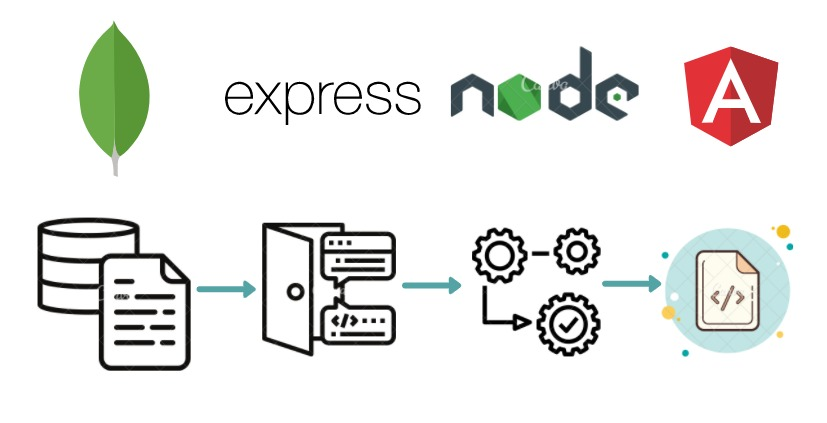
\includegraphics[width=0.99\textwidth]{meanstack}};



\end{frame}


\begin{frame}{Why MEANSTACK?}
	\begin{columns}
		\begin{column}{5cm}
			\begin{center}
				
\includegraphics[height=6cm]{chamaeleon_hochformat}
				
				{\tiny \textcolor{digiPH_darkorange}{ }}
			\end{center}
		\end{column}
		\begin{column}{5cm}
			\begin{center}
				\Large
			
			\end{center}
			
		\end{column}
	\end{columns}
\end{frame}



\begin{frame}{Features and API's}
	
	\begin{center}
	

\begin{itemize}
\item Contact form
\item Maps
\item Chat-bot
\item News API 
\item Image upload
\end{itemize}

\columnbreak


\begin{itemize}
\item Message sending
\item Certificate Download
\item Video call
\end{itemize}
\end{center}
\end{frame}



\begin{frame}{Our features look like ...}
	\begin{columns}
		\begin{column}{5cm}
			\begin{center}
				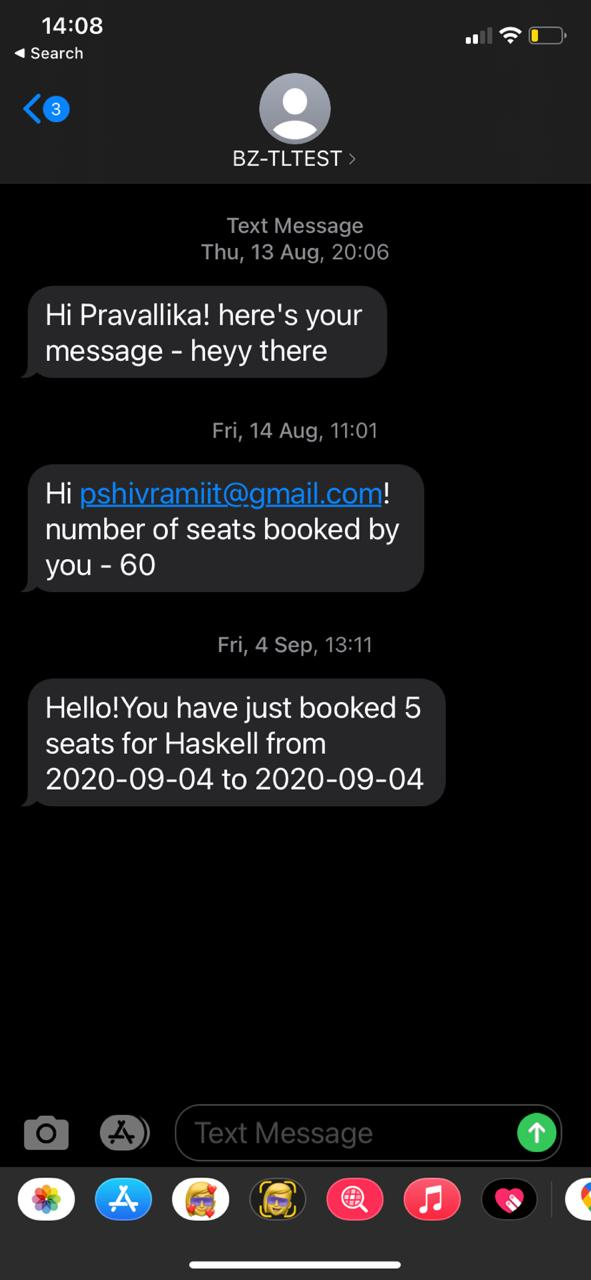
\includegraphics[height=7cm]{message}
				
				{\tiny \textcolor{digiPH_darkorange}{ }}
			\end{center}
		\end{column}
		\begin{column}{5cm}
			\begin{center}
				\Large
			
			\end{center}
			
		\end{column}
	\end{columns}
\end{frame}



\begin{frame}{Our features look like ...}
	\begin{columns}
		\begin{column}{5cm}
			\begin{center}
				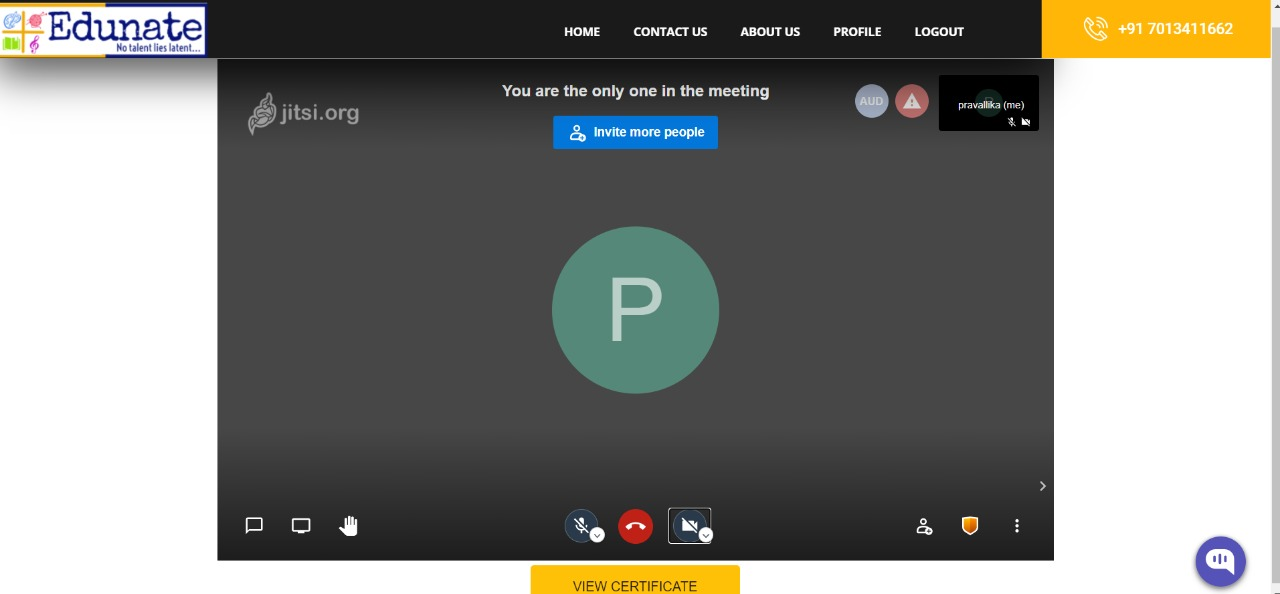
\includegraphics[height=5cm]{video}
				
				{\tiny \textcolor{digiPH_darkorange}{ }}
			\end{center}
		\end{column}
		\begin{column}{5cm}
			\begin{center}
				\Large
			
			\end{center}
			
		\end{column}
	\end{columns}
\end{frame}



\begin{frame}{Our features look like ...}
	\begin{columns}
		\begin{column}{5cm}
			\begin{center}
				
\includegraphics[height=5cm]{certificate}
				
				{\tiny \textcolor{digiPH_darkorange}{ }}
			\end{center}
		\end{column}
		\begin{column}{5cm}
			\begin{center}
				\Large
			
			\end{center}
			
		\end{column}
	\end{columns}
\end{frame}



\begin{frame}{Our features look like ...}
	\begin{columns}
		\begin{column}{5cm}
			\begin{center}
				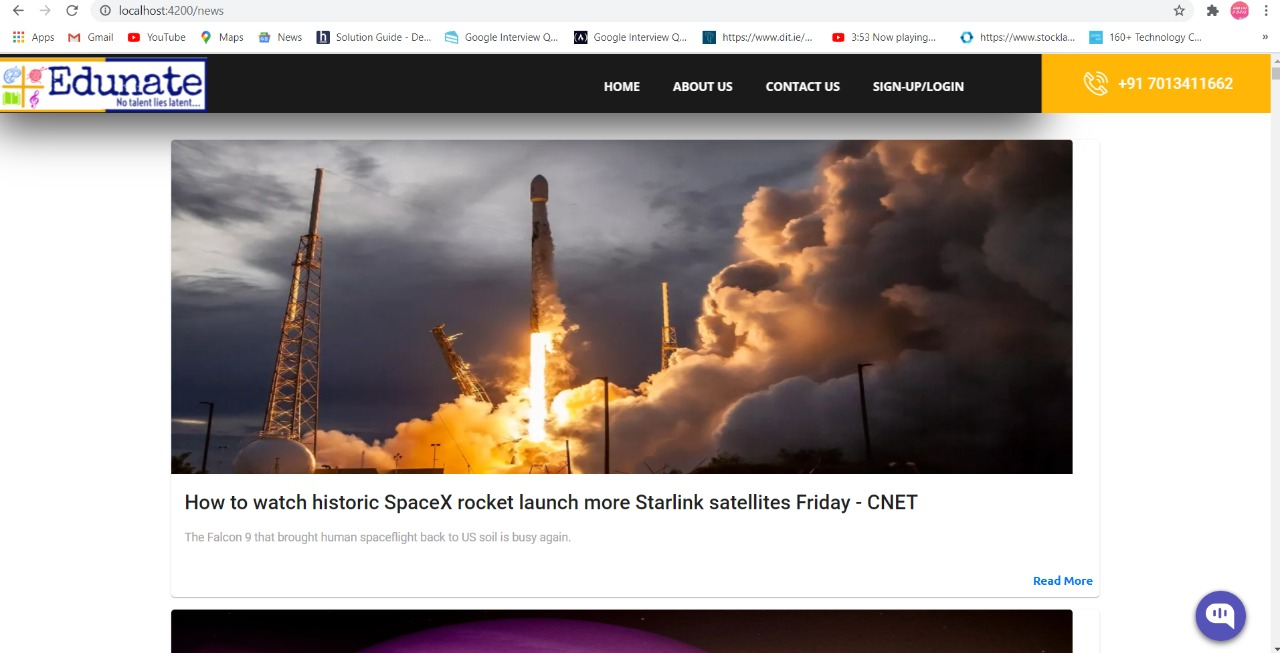
\includegraphics[height=5cm]{news}
				
				{\tiny \textcolor{digiPH_darkorange}{ }}
			\end{center}
		\end{column}
		\begin{column}{5cm}
			\begin{center}
				\Large
			
			\end{center}
			
		\end{column}
	\end{columns}
\end{frame}



\begin{frame}{Our features look like ...}
	\begin{columns}
		\begin{column}{5cm}
			\begin{center}
				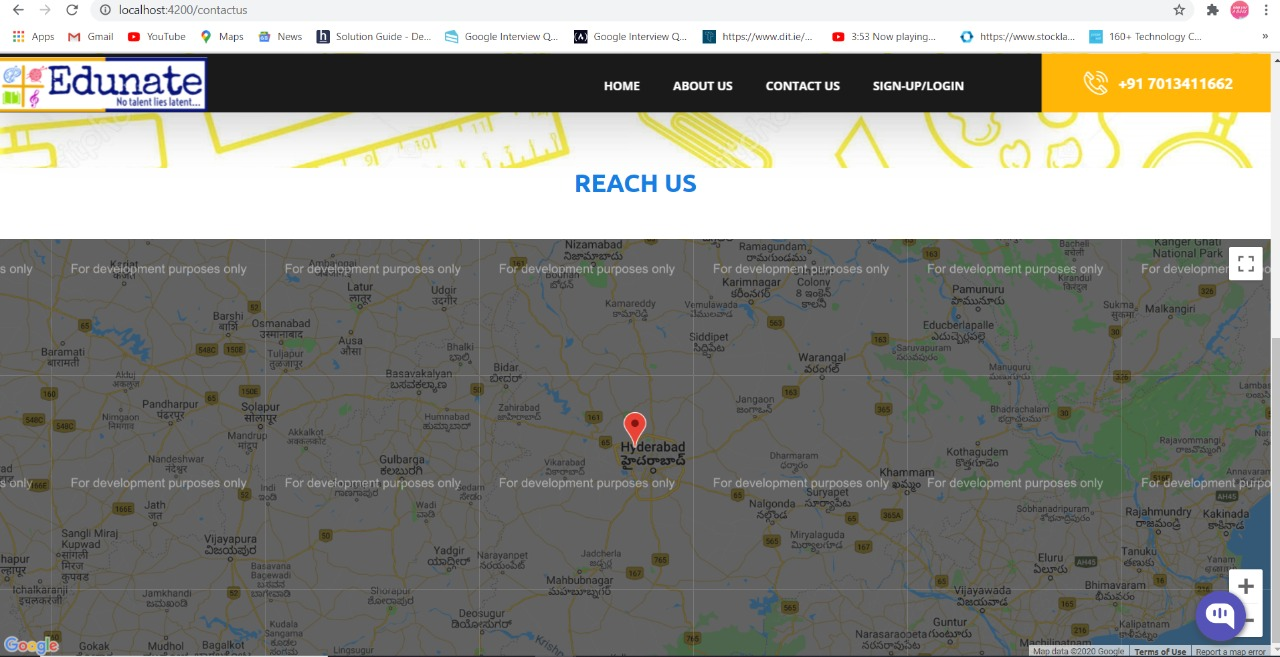
\includegraphics[height=5cm]{maps}
				
				{\tiny \textcolor{digiPH_darkorange}{ }}
			\end{center}
		\end{column}
		\begin{column}{5cm}
			\begin{center}
				\Large
			
			\end{center}
			
		\end{column}
	\end{columns}
\end{frame}



\begin{frame}{Our features look like ...}
	\begin{columns}
		\begin{column}{5cm}
			\begin{center}
				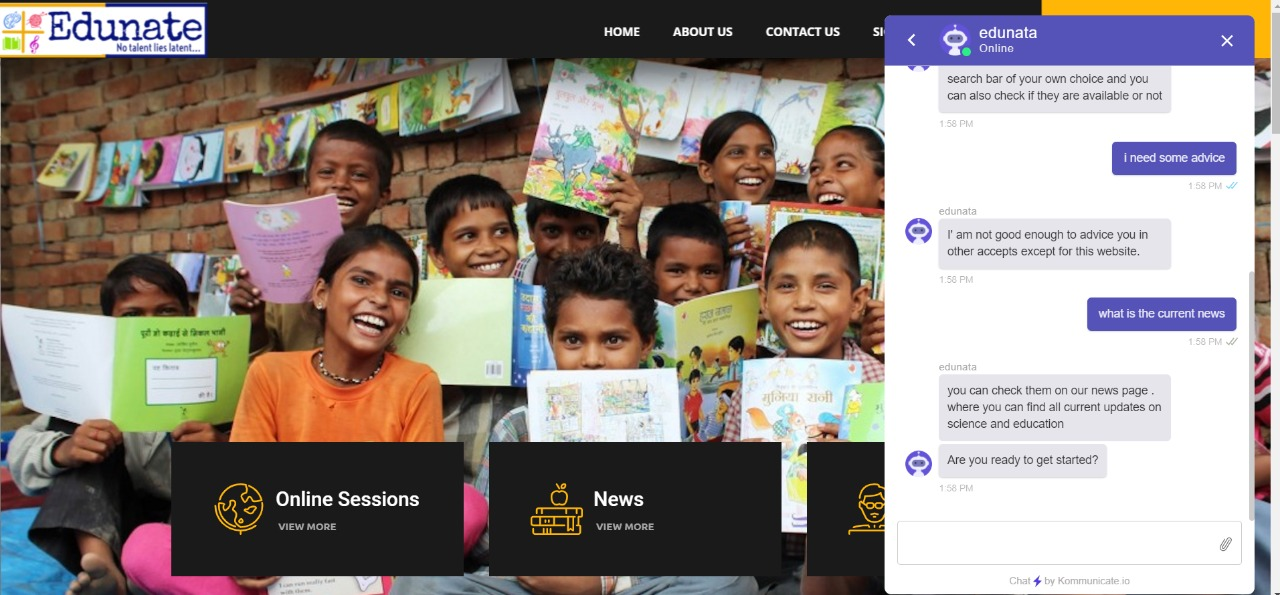
\includegraphics[height=5cm]{chatbot}
				
				{\tiny \textcolor{digiPH_darkorange}{ }}
			\end{center}
		\end{column}
		\begin{column}{5cm}
			\begin{center}
				\Large
			
			\end{center}
			
		\end{column}
	\end{columns}
\end{frame}



\begin{frame}{Hurdles faced \ldots}
	\framesubtitle{}
	\begin{center}
		\begin{tikzpicture}
			\node[anchor=south west,inner sep=0] (bild) at (0,0) {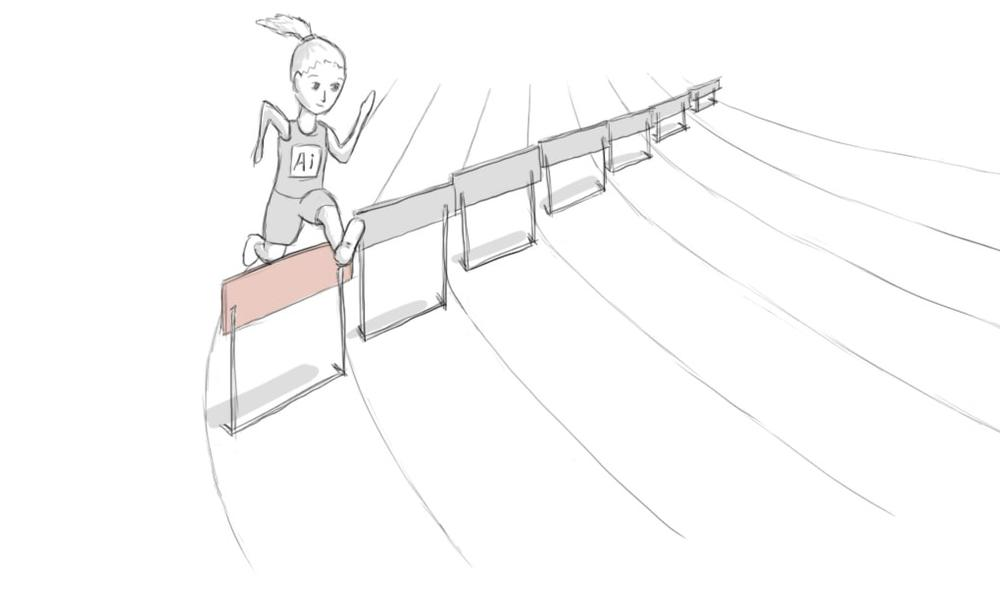
\includegraphics[width=0.99\textwidth]{smartphone}};
			\begin{scope}[x=(bild.south east),y=(bild.north west)]
				% Gitternetz einzeichnen
				%\draw[help lines] (0,0) grid[xstep=0.1,ystep=0.1] (1,1);
				% Text einfügen
				\node[font=\scriptsize,align=left,color=white,text width=4cm] (text) at (0.79,0.3) {Bitte verwenden Sie ausschließlich urheberrechts-einwandfreies Bildmaterial (NoGo: Schulbücher!)\\
				Am besten also: eigenes und/oder CC-Bildmaterial, \zB von \url{www.pixabay.com} oder ähnlichen Plattformen!\\
				Bitte nie eine sichtbare Bildquelle und Lizenz vergessen.};
			\end{scope}
		\end{tikzpicture}
		
			\end{center}
\end{frame}
\begin{frame}	\begin{center}
		\Huge
Find us at \color{blue} \url{https://github.com/pravallika-1305/EDUNATE}
	\end{center}
\end{frame}

\begin{frame}{Lets have a look!!}
	\begin{columns}
		\begin{column}{5cm}
			\small 
		\end{column}
		\begin{column}{5cm}
			\begin{center}
				
\includegraphics[height=3cm]{details_foto_xy2}
				
				
			\end{center}
		\end{column}
	\end{columns}
	\begin{columns}
		\begin{column}{5cm}
			\begin{center}
				
\includegraphics[width=5cm]{details_foto_xy1}
				
				
			\end{center}
		\end{column}
		\begin{column}{5cm}
			\begin{block}{\small }
				\scriptsize
				
			\end{block}
		\end{column}
	\end{columns}
\end{frame}


\begin{frame}{Our Team}
	\begin{columns}
		\begin{column}{0.25cm}
			\begin{center}
				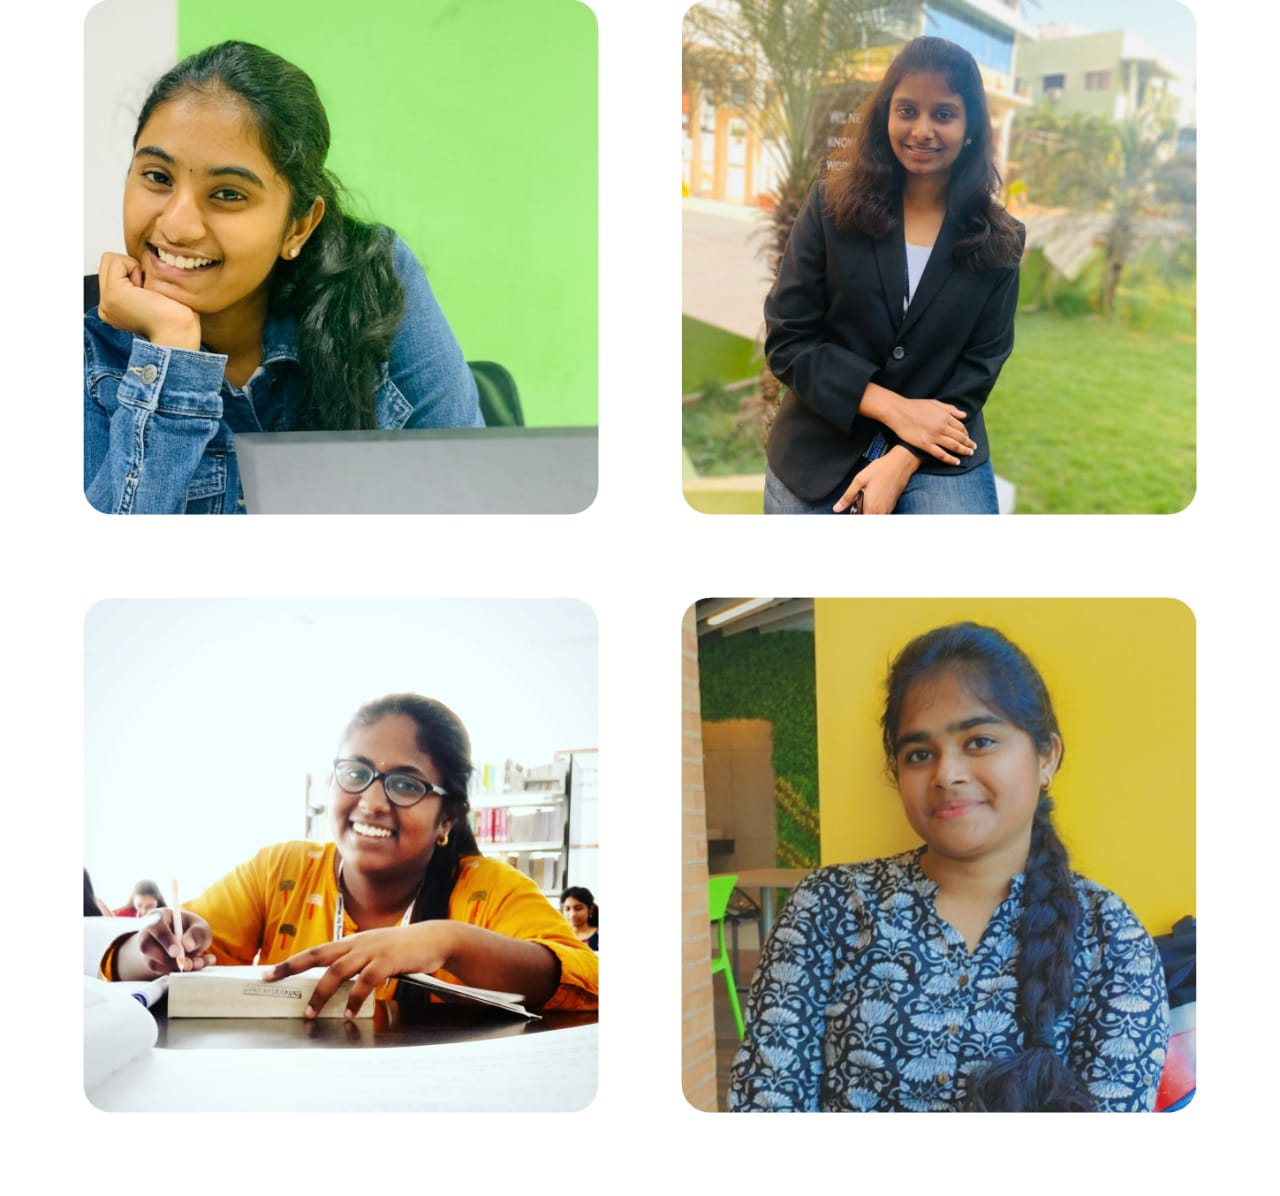
\includegraphics[scale = 0.5,width=8cm,height=8cm]{ourteam1}
				
				{\tiny \textcolor{digiPH_darkorange}{ }}
			\end{center}
		\end{column}
		\begin{column}{5cm}
			\begin{center}
				\Large{}
			
			\end{center}
			
		\end{column}
	\end{columns}
\end{frame}



\end{document}
